%!TEX root = main.tex
\section{Experimental Setup\label{sec:experiment_setup}}

\subsection{Dataset Description\label{dataset}}
\par \noindent We collected crowdsourced segmentations from Amazon Mechanical Turk; each HIT consisted of one segmentation task for a specific pre-labeled object in an image. There were a total of 46 objects in 9 images from the MSCOCO dataset~\cite{Lin2014} segmented by 40 different workers each, resulting in a total of 1840 segmentations. Each task contained a keyword for the object and a pointer indicating the object to be segmented. Two of the authors generated the ground truth segmentations by carefully segmenting the objects using the same task and interface. 
\par A sub-sampled dataset was created from the full dataset to determine the efficacy of these algorithms on varying number of worker responses. Every object was randomly sampled worker with replacement. For small worker samples, we average our results over larger number of batches than for large worker samples (which have lower variance, since the sample size is close to the original data size).

\subsection{Evaluation Metrics}
\par \noindent Evaluation metrics used in our experiments measure how well the final segmentation (S) produced by these algorithms compare against ground truth (GT). The most common evaluation metrics used in the literature\cite{Cabezas2015,Sameki2015,Song2018,Lin2014} are area-based methods that take into account the intersection area, $IA=area(S\cap GT)$, or union area, $UA=area(S\cup GT)$ between the worker and ground truth segmentations, including %. Specifically, we use
    $\text{Precision (P)} = \frac{IA(S)}{area(S)}$, 
    $\text{Recall (R)} = \frac{IA(S)}{area(GT)}$, and 
    $\text{Jaccard (J)} = \frac{UA(S)}{IA(S)}$.
    %metrics to evaluate our algorithms.
\subsection{Baseline Algorithms}
\subheading{Retrieval-based Methods}

\par \noindent\textbf{Number of Control Points (num pts)}: This algorithm picks the worker segmentation with the largest number of control points around the segmentation boundary (i.e., the most precise drawing) as the output segmentation \cite{Vittayakorn2011,Sorokin2008}. Intuitively, workers that have used a larger number of points are likely to have been more precise, and provided a more complex and accurate segmentation. 
\par \noindent\textbf{Average worker}: This baseline computes the average Jaccard across all workers, which simulates collecting only a single worker annotation.
\par \noindent\textbf{Best worker}: Selecting the best worker based on Jaccard against ground truth. 

\subheading{Vision-based Methods~\label{sec:vision}}

\par We implement a semi-supervised algorithm that can produce segmentations for arbitrary objects in the absence of large volumes of tailor-made training data. While this algorithm works largely on raw image data, it requires some external help in the form of one ``reference'' segmentation. Intuitively, a rough segmentation can be thought of as a pointer for the algorithm to the relevant regions of the image. The algorithm then uses the color profile of the image to segment out the similarly colored regions of the image that overlap with the reference segmentation. Specifically, we begin by splitting the input image into multiple regions, or {\em tiles} that have the same color using the work of~\cite{felzenszwalb2004efficient}---the desired number of output tiles can be modified using a tuning parameter $k$, to produce finer or coarser tiles.

We used the popular open source segmentation algorithm developed by Felzenszwalb and Huttenlocher~\cite{felzenszwalb2004efficient}. We fixed the smoothing and minimum component size parameters and varied the threshold determining the how refined the segmentation is. As shown in Figure~\ref{vision_example}, larger values for k result in larger components in the result. We overlay the given rough segmentation on top of the color tiles.

\begin{figure}
\vspace{-30pt}
\centering
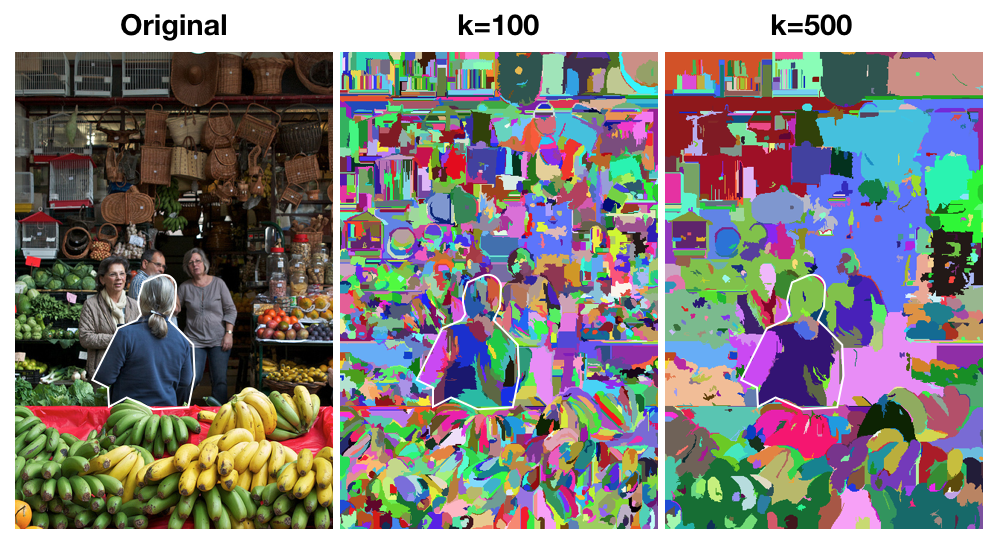
\includegraphics[width=0.9\linewidth]{plots/vision_tiles.png}
\caption{Example of the vision color tiling for different chosen granularities. Left: Raw image. Vision segmentation with $k=100$(Center) and $k=500$ (Right). Vision tiles with a significant overlap area with the worker segmentation (white boundaries) is selected.}
\label{vision_example}
\end{figure}

\par \noindent\textbf{Average vision}: 
\par \noindent\textbf{Best vision}: 
Now, the algorithm focuses on {\em choosing the right set of tiles based on the given reference segmentation}. 
Intuitively the algorithm picks color tiles that have significant overlap with the given reference segmentation, i.e., returns the union of all tiles for which greater than a certain area threshold of the tile is intersecting with the reference segmentation. We experiment with different granularities for the vision preprocessing as well as scan a variety of tile filtering area thresholds. 